\documentclass[a4paper,12pt]{article}
\usepackage[utf8]{inputenc}
\usepackage{geometry}
\geometry{a4paper, total={160mm,257mm}, left=25mm, top=20mm}

\setlength{\parindent}{0em}
\setlength{\parskip}{1em}
\renewcommand{\baselinestretch}{1.15}

\usepackage{xcolor}

\usepackage{array}

\usepackage{verbatim}

\usepackage{listings}
\lstset{breaklines=true}


\usepackage{graphicx} 

\graphicspath{ {images/} }

\usepackage{hyperref}

\title{Learning Journal}
\author{Andrew White}
\date{Semester 2 - 2019}



\begin{document}

\maketitle

\tableofcontents

\newpage

The purpose of this journal is to document the objective, action, errors and results of tasks set for the FOAR705 Unit. The Journal is being done in LeTeX, which will be a good learning exercise for myself, as someone who has never used LaTeX before. 

\section{Week 1}
\subsection{Install Software} 

\noindent \textbf{Objective:} Install software Rstudio, Slack and login to Cloudstor and Github \\

\noindent \textbf{Action:} download \verb|rstudio-1.2.1335-x86_64.rpm| from the RStudio website and use the wget command to download Slack. Logged on to Cloudstor and created a github account without any problems. Github user name is a-white42\\\

\noindent install using: rpm -U \verb|rstudio-1.2.1335-x86_64.rpm|\\

\noindent wget \verb|https://downloads.slack-edge.com/linux_releases/slack-3.4.0-0.1.fc21.x86_64.rpm|\\

\noindent sudo dnf localinstall \verb|slack-3.4.0-0.1.fc21.x86_64.rpm|\\

\noindent \textbf{Errors:} RStudio returns an error message because R programming language is not installed on my system.\\

\noindent \textbf{Action:} sudo yum install R\\

\noindent \textbf{Result:} RStudio runs perfectly. 

\section{Week 2}

\subsection{Restore Backup}

\noindent \textbf{Objective:} Restore a file from a 6 month or older backup. Document how it goes.\\

\noindent \textbf{Action:}  The intention of this action is to see if I can successfully restore and read a backup that is over 6 months old. The process involved a manual search of my external hard drives searching for an older project and copying a drawing into my current projects directory.\\

\noindent \textbf{Errors:} None.. 

\noindent \textbf{Result:} The restore was successful and I was able to open the drawing in AutoCAD without any errors.

\subsection{LaTeX}

\noindent \textbf{Objective:} I have decided to use LaTeX for my Learning Journal to force myself to learn LaTeX and hopefully through the process develop a better understanding. I would like to be able to use LaTex to write some papers so learning footnotes will be key to this.\\ 

\noindent \textbf{Action:} I have Currently installed two LaTeX editors on my Fedora system, however, I am starting with Overleaf as it seems like a good starting point. Overleaf provides a nice preview, which GNOME LaTeX and TeXStudio do not seem to (or I just do not understand how to configure it to do this yet), it also has lots of templates and while I am trying to avoid templates for the purpose of learning it will be useful to see what is possible and how you might go about achieving a desired result.

I created a basic LaTeX document in Overleaf using the Source tab so that I can become familiar with several of the basic commands.\\

\noindent \textbf{Errors:} I have discovered, through error that the backslash end{document} command does not end the section but ends the document and having two of these in the TeX file causes a wee little problem.\\  

\noindent \textbf{Result:} I have written the first two journal entries and have a few comments. I need a better understanding of how to set out the document. Currently I am using the section command for week entries and the subsection command for different content. This might not be the best way to do this but seems okay for now.\\

\subsection{Some useful LaTex Commands} 

\begin{verbatim}
\textit{text in italics} 
\underline{text underlined}
\textbf{text in bold}
\large {large words}\\
\\ forces a new paragraph
\vspace{5mm} makes a space between lines of a specified amount.
\noindent if you don't want an indent at the begining of a paragraph.
\normalsize normal size font
\small small font
\large large font
\tiny tiny font

\end{verbatim}

Examples:

\textit{text in italics} 
\underline{text underlined}
\textbf{text in bold}
\large {large words}\\

\vspace{5mm}
LaTeX produces two kinds of {\textbf{lists}}. \textbf{enumerate} produces numbered lists and \textbf{itemize} produces bullet point lists. Here is an example.
\begin{enumerate}
\item First numbered item
\item Second numbered item
\begin{itemize}
\item First bullet point
\item Second bullet point
\end{itemize}
\item Third numbered item
\end{enumerate}

\noindent \textbf{Error:} The Large text command I entered above was still active. To fix this I needed to reinstate the \textbackslash normalsize font command.

\vspace{5mm}

\normalsize 

In order to use hyperlinks in LaTex, we have to import the hyperref usepackage in the preamble of the document. \verb|\usepackage{hyperref}| It is recommended that this is the last package to get loaded otherwise it could cause problems.

Example: Hyperlink opens in a new page.

\url{https://www.overleaf.com/learn/latex/Page_size_and_margins}

\subsection{Data Carpentry}

\noindent \textbf{Objective:} Complete Data Carpentry called Data Organization in Spreadsheets for Ecologists found at \url{https://datacarpentry.org/spreadsheet-ecology-lesson/}\\

\noindent \textbf{Action:} Finished all 6 lessons\\

\noindent \textbf{Errors:} No Errors\\

\noindent \textbf{Result:} Notes kept in Joplin for future reference. \\

\newpage

\section{Week 3}

\subsection{LaTeX Scoping Exercise}

\noindent \textbf{Objective:} While doing the scoping exercise I needed to add a table to demonstrate a spreadsheet layout concept.\\

\noindent \textbf{Action:} I did some reading and discovered that there are several ways to add tables, however, I good suggested method is to load \verb|\usepackage{array}| in the preamble. The section of a TeX document between\verb|\documentclass{...} and \begin{document}| is called the preamble. This section normally contains commands that affect the entire document such as setting document type, paper size, fonts, margins, etc...\\

\noindent \underline{This is a sample table}
\begin{center}
\begin{tabular}{ | m{2.5cm} | m{6cm}| m{6cm} | } 
\hline
Column 1 & Column 2 & Column 3 \\ 
\hline
Text 1 & Text 2 & Text 3 \\ 
\hline
\end{tabular}
\end{center}

\noindent \textbf{Errors:}  I encountered some errors initially such as the table was going off the page. This was fixed with the addition of the \verb|\usepackage{array}|\\ 

\noindent \textbf{Result:} I was able to successfully add a table to my Scoping Exercise.
You can add footnote with the \textbackslash footnote command \footnote{Footnotes are added using \textbackslash footnote, with the footnote content in curly brackets.}

\subsection{BibTeX}

\noindent \textbf{Objective:} get BibTeX working in my Scoping exercise as a proof of concept. 

\noindent \textbf{Action:}: Created a BibTex filed called ref01.bib with a sample entry.
Added the bibliography commands to my LaTex document.
\begin{verbatim}
\bibliography{ref01.bib}
\bibliographystyle{ieeetr} The ieeetr variable is the citation style. 
\end{verbatim}
\noindent \textbf{Errors:} None... I was actually very surprised that I got this to work without any dramas.

\noindent \textbf{Result:} I am happy with this result. I can now create an independent bibliography file and reference it from within a LaTeX document. I found also that the cite button on google scholar also has a function to create BibTeX code which you can copy/paste into the bibliography.bib file. 

\newpage

\section{Week 4}

\underline {Things to do}

\begin{enumerate}
\item Do all data carpentry exercises.
\item Export the csv. View it in a text editor like Atom.io, Sublime Text, or notepad++ Think about the benefits of an always-readable and not tied to a subscription or specific program data format
\item Proof of Concept assignment 
\item I found lessons on Version Control with Git http://swcarpentry.github.io/git-novice/
\end{enumerate}

\subsection{Data Carpentry}

Since I finished the data carpentry exercises in week 2, I though I would review the dates as data lesson and test exporting CVS data.

\noindent \textbf{Objective:} Data Carpentry Dates as data

Important tip, write the month part of your date as letters so there is no confusion which date format you are using. 

The ISO 8601 standard is YEAR-MONTH-DAY

\noindent \textbf{Errors:} None..

\noindent \textbf{Result:} Successfully completed Data Carpentry exercises and exported CVS data. Note, CVS data loses all formatting such as colours, column width and height information as well as data validation. 

\subsection{Scoping Exercise II}

\noindent \textbf{Objective:} Complete Scoping Exercise II in LaTeX

\noindent \textbf{Action:}:Create Scoping Exercise II in LateX using my previous Create Scoping Exercise I LaTeX document as a template. Added some addition formatting to improve the layout including usepackage fancyhdr

\noindent \textbf{Errors:} Package Fancyhdr Warning: \textbackslash headheight is too small (12.0pt): Make it at least 13.59999pt. We now make it that large for the rest of the document. This may cause the page layout to be inconsistent, however.

\noindent \textbf{Result:} Scoping Exercise II created successfully with the expect of this error which needs some further problem solving.
 
\newpage

\section{Week 5}

\underline {Things to do this week}
 
Set work:
\begin{enumerate}
    \item Work on: http://swcarpentry.github.io/shell-novice/ and do episodes : Introduction, Navigating Files and Directories, Working with Files. Put results into a new (or new section, or otherwise demarcate them) learning journal.
    
    I should do some additional unix learning here since I have been a unix/linux user since 1993. I will see how it goes since you always pick up something new when revising old material. 
    
    \item Finish Elaboration I. This is due in cloudstor only before the Week 5 class (though it will form part of your Elaboration II submission). Commit to git as you are committing all assignments, in whatever organisation you choose. 

\end{enumerate}

Other work:

I have neglected learning how to commit my journal in Overleaf to github automatically. I searched Slack and found Brian's post on this procedure.\\

\url{https://www.overleaf.com/learn/how-to/How_do_I_connect_an_Overleaf_project_with_a_repo_on_GitHub,_GitLab_or_BitBucket%3F}\\

\subsection{Configure Overleaf to commit to github}

\textbf{Objective:} Configure Overleaf to commit to github

\textbf{Action:} Read info from Brain's post. From Menu in Overleaf, select github and create a repository. Select MQ-FOAR705 and create a repo called \verb|Andrew_White-Learning_Journal|. Commit changes to github

\textbf{Errors:} I think I should have committed this to a sub-folder under a-white42-Exercises so that all my work is in a central file. 

\textbf{Results:} My journal commited to github without any errors. I should ask Brian about moving the \verb|Andrew_White-Learning_Journal| folder.



There are three steps to effective bibliography management:

    Creating a .bib file.
    Insert references into your .tex file.
    Format your references.

\newpage

\subsection{Data Carpentry - The Unix Shell}

\textbf{Objective} There is a 2 others ways to return to the home directory than cd or cd /home/andrew. typing cd \verb|~| (tilde) or cd \verb|$HOME| will also produce the same result. :

\textbf{Action:} tested commands. 

\textbf{Errors:} No errors with the command however the tilde character is not displayed in the LaTeX PDF file. The solution is the add the verb command. 

\textbf{Results:} Commands work fine, and LaTeX processed correctly.


\textbf{Objective} create a LaTeX document in the command line. 

\textbf{Action:} make directory, change directory, make file, run vi, type in LaTeX code, exit and display code. 

\begin{verbatim}
[andrew@superman ~]$ mkdir thesis
[andrew@superman ~]$ cd thesis
[andrew@superman thesis]$ pwd
/home/andrew/thesis
[andrew@superman thesis]$ ls -l
total 4
-rw-rw-r--. 1 andrew andrew 0 Aug 29 14:09 thesis.tex
[andrew@superman thesis]$ touch thesis.tex
[andrew@superman thesis]$ vi thesis.tex 
[andrew@superman thesis]$ ls -l
total 4
-rw-rw-r--. 1 andrew andrew 192 Aug 29 14:09 thesis.tex
[andrew@superman thesis]$ cat thesis.tex

\documentclass[11pt]{article}
\usepackage[utf8]{inputenc}

\title{test thesis}
\author{Andrew White}
\date{}

\begin{document}

\maketitile

\section{section 1}

This is a test document. 

\end{document}
\end{verbatim}

run pdflatex thesis.pdf

\textbf{Errors:} pdflatex returned the following error in the thesis.log file.

\begin{verbatim}
This is pdfTeX, Version 3.14159265-2.6-1.40.19 (TeX Live 2018) (preloaded format=pdflatex)
 restricted \write18 enabled.
entering extended mode
(./thesis.tex
LaTeX2e <2018-04-01> patch level 5
(/usr/share/texlive/texmf-dist/tex/latex/base/article.cls
Document Class: article 2014/09/29 v1.4h Standard LaTeX document class
(/usr/share/texlive/texmf-dist/tex/latex/base/size11.clo))
(/usr/share/texlive/texmf-dist/tex/latex/base/inputenc.sty)
Runaway argument?
{document 
! Paragraph ended before \begin was complete.
<to be read again> 
                   \par 
l.10 
     
? ^C! Interruption.
l.10 
\end{verbatim}
The problem was I was missing a curly bracket. This is what happen when you type everything in manually. 

\textbf{Results:} Fixed curly bracket and document generated thesis.pdf file correctly. 

\textbf{Errors:} I initially used the \verb|\verbatim| and \verb|\endverbatim| commands but these returned errors. I fixed this with the \verb|\begin{verbatim} \end{verbatim}| command instead. 


\subsection{LaTeX Error: hbox badness 10000}

\textbf{Objective:} I keep getting this error in LaTeX:\\ 

\verb|Underfull \hbox (badness 10000) in paragraph at lines 48--49|

\textbf{Action:} Online I read that, An underfull hbox means LaTeX couldn't space the line wide enough to fill the entire width of the page, without increasing word spacing beyond the allowed maximum;

One suggested fix is to include \verb|\hbadness=99999| in the preample because it is greater than 10000. 

\textbf{Errors:} no errors when I added \verb|\hbadness=99999|

\textbf{Results:} This seems like a patch for a problem that maybe shouldn't be there. It might something I have done and I should test the document to see if I can locate the source, or the correct way to set up the preample so this doesn't orrur. 



\subsection{Data Carpentry - The Unix Shell 2}

\textbf{Objective:} Creating aliases. Aliases let you define commands or shortcuts. For example, \textbf{alias lm="ls -al|more"} defines the alias command lm to run the ls command with arguments -a and -l and the more option to pause at the end of each page.

\textbf{Action:} Test alias and add to .bashrc
\begin{enumerate}
    \item Start with the \textbf{alias} command
    \item Type the name (shortcut) of the alias you want to create
    \item Then an = sign, with no spaces on either side of the =
    \item Then type the command (or commands) you want your alias to execute when it is run. 

\end{enumerate}

In a terminal,  run \textbf{alias lm="ls -al|more" } and test. Then edit .bashrc with the vi text editor and add alias lm="ls -al|more" under the section for \textit{User specific aliases and functions }so this alias is available every time I run a terminal window.  


\textbf{Errors:} none.. 

\textbf{Results:} Tested fine by running a new terminal window and confirmed.

Just for fun, I set the allowing alias to open firefox in a new window at the url for overleaf.

\verb|alias ol="firefox --new-window https://www.overleaf.com/project"|

\section{Week 6}

\subsection{Data Carpentry - General}

\textbf{Notes:} Useful information

When working in a terminal, it is handy to use the [TAB] key to fill out the rest of a file or directory name.\\

e.g. mv slack[TAB] Dow[TAB] will follow with mv \verb|slack-4.0.2-0.1.fc21.x86_64.rpm Downloads|

This works with directories also. 

when working in Overleaf and you accidentally delete something, CTRL+z will undo. CTRL+f find and replace

Handy Hotkeys for overleaf \url{https://www.overleaf.com/learn/how-to/Hotkeys}

\subsection{Data Carpentry - Unix Shell 3}

\textbf{Objective:} Test out wc command 

\textbf{Action:} Tested wc command with TXT files and also PDF. I suspected that PDF would not work since they are based on postscript and not ASCII text files. Nevertheless, I thought it was worth testing to see what happens.  

\textbf{Errors:} The PDF files returned incorrect numbers. I pdf file with 1400 words returned 2500 words.

\textbf{Results:} wc command works well for comparing text files and will be usefil for LaTeX files since these are in plain text format.


\subsection{Fedora 30 desktop}
\textbf{Objective:} Install a dual boot fedora system on my desktop. The purpose of this exercise is to firstly, to set up a new system and document it and secondly, to test out some LaTeX commands such as subsubsection, url, and how to layout an instruction to setup a system in the future. \\

\textbf{Action:} Install a typical installation of fedora from a usb image. 

Post installation: These are things to do after installing Fedora. Commands will vary depending on the Linux distribution.  

\subsubsection{Update System}   

\verb|$ sudo dnf update|

\subsubsection {Enable RPM Fusion Repositories}
RPM fusion repertories homepage is \url{https://rpmfusion.org/} RPM Fusion provides software that the Fedora Project or Red Hat doesn't want to ship. That software is provided as precompiled RPMs for all current Fedora versions and current Red Hat Enterprise Linux or clones versions; you can use the RPM Fusion repositories with tools like yum and PackageKit.

There are two repositories on rpm fusion, a free repository and a non-free repository. 

\verb|$ sudo dnf update --refresh|

\verb|$ sudo dnf install https://download1.rpmfusion.org/free/fedora/rpmfusion-free-release-$(rpm -E %fedora).noarch.rpm |

\verb|$ sudo dnf install https://download1.rpmfusion.org/nonfree/fedora/rpmfusion-nonfree-release-$(rpm -E %fedora).noarch.rpm|

\subsubsection{Player and Codecs}

\verb|$ sudo dnf install youtube-dl vlc|

\begin{verbatim}$ sudo dnf install \
gstreamer-plugins-base \
gstreamer1-plugins-base \
gstreamer-plugins-bad \
gstreamer-plugins-ugly \
gstreamer1-plugins-ugly \
gstreamer-plugins-good-extras \
gstreamer1-plugins-good \
gstreamer1-plugins-good-extras \
gstreamer1-plugins-bad-freeworld \
ffmpeg \
gstreamer-ffmpeg
\end{verbatim}

\subsubsection{Gnome tweak tool}

\verb|$ sudo dnf install gnome-tweak-tool|

\subsubsection{Compression and archiever tools}

\verb|$ sudo dnf install unzip p7zip|

\subsubsection{Install vlc media player}

\verb|$ sudo dnf -y install vlc|

\subsubsection{Install Wunderlistux}

Wunderlistux is a to-do list application. Project found at \url{https://github.com/edipox/wunderlistux}

\verb|$ cd ~/Downloads|

\verb|$ wget https://github.com/edipox/wunderlistux/releases/download/Linux-0.0.8/Wunderlistux-0.0.8.rpm|

\verb|$ sudo dnf install Wunderlistux-0.0.8.rpm|

\subsubsection{GNU Image Manipulation Program}

Gimp image editing software. Project found at \url{https://www.gimp.org/}

\verb|$ sudo dnf install gimp|

\subsubsection{Stacer} 

Stacer is a Linux System Optimizer and Monitoring tool. 

Project is found on github at: 

\url{https://oguzhaninan.github.io/Stacer-Web/} and  \url{https://github.com/oguzhaninan/Stacer}

\verb|$ wget https://github.com/oguzhaninan/Stacer/releases/download/v1.0.8/stacer-1.0.8_x64.rpm|

\verb|$ dnf install stacer-1.0.8_x64.rpm|

\subsubsection{Shutter}

Shutter is a feature-rich screenshot program. You can take a screenshot of a specific area, window, your whole screen, or even of a website - apply different effects to it, draw on it to highlight points, and then upload to an image hosting site, all within one window.

\verb|$ sudo dnf -y install shutter|

\subsubsection{R Programming Language and RStudio}

\verb|$ sudo dnf install R|

Download RStudio from the RStudio website

\verb|$ sudo dnf install rstudio-1.2.1335-x86_64.rpm|

\textbf{Errors:} An error worth noting. When downloading Stacer using wget, I accidentally run the sudo (superuser do) command so the rpm was downloaded and permissions assigned to the root account. 

i.e.
\begin{verbatim}
[andrew@batman Downloads]$ ls st* -l
-rw-r--r--. 1 root root 23926761 Aug 23  2017 stacer-1.0.8_x64.rpm
\end{verbatim}

\textbf{Results:} System up and running. Tested installed software and everything seems to work. 

\newpage

\section{Week 7}

\subsection{Open Refine}

Open Refine is a standalone open source desktop application for data cleanup and transformation to other formats, the activity known as data wrangling. 

terms: clustering, data wrangling, GREL (General Refine Expression Language).

Problem: there might be a column where an entry is spelt 3 ways. 

\subsection{Open Refine Import and Filtering and Sorting}


%% \textbf{Action:}
%% \textbf{Errors:}
%% \textbf{Results:}

\textbf{Objective:} Import ILO time-related underemployment data into OpenRefine and export only Australian data for the 15-24 year old age group. 

\textbf{Action:} 

Download time-related underemployment data from the International Labour Organization.

Open new project in OpenRefine

Load \verb|MBI_18_EN,xlsx|

The spreadsheet contains 4472 entries (rows). From the column listed as time-related-underemployment select text filter and type in Australia. The spread sheet filters out all entries expect the 76 entries for Australia.  

Next add text facet to column 3 and select only the 15-24 age groups.

Export to CSV file and open in Libre Office. 

\textbf{Errors:} None.

\textbf{Results:}

The CSV file now contains only the data for time-related-unemployment in Australia for the 15-24 year old age group.

\subsection{Examining Numbers in OpenRefine}

\textbf{Objective:} Transform three more columns, from text to numbers. Can all columns be transformed to numbers? 

\textbf{Action:} Select Edit Cell, Common Transforms and then To number for each column.  

Columns with number data can be transformed to a number. Columns with text data, such as \verb|respondent_wall_type| or village cannot be transformted to numbers.

\textbf{Errors:}  Text transform on 0 cells in column village: value.toNumber() Undo 

\textbf{Results:} Only the data in the columns containing numbers was transformed. 

\textbf{Action:} Replaced one numeric cell on the years farmed column with the text abc. Select numeric facet from the pull down menu. On the left panel there are several check boxes Numeric, Non-numeric, Blank, and Error. There are 130 enrties for numeric and only 1 entry for non-numeric. De-selecting the tick box for the non-numeric option turns off the corresponding row. 

\textbf{Results:} Now the selection contains only the rows that contain numbers in the years farmed column. 

\subsection{Proof of Concept Notes}

As a [role], I want [goal] so that [reason].
As a [masters student], I want [suitable word processor] so that [write my thesis].

\subsection{Bibliography}

\textbf{Objective:} Install bibliography in my learning journal so I an either reference weekly readings or record them for future reference. 

\textbf{Action:} Created \verb|foar705_biblio.bib| Then copied in the BibTeX citation data for the 3 required readings for this week. Data was taken from the browzine interface for the nature articles and the \textbf{Art of Software Testing (3rd Edition)} taken from the digital source, Knovel website. 

Added LaTeX commands to learning journal:

\begin{verbatim}
\newpage
\nocite{*} 
\bibliography{foar705_biblio.bib}
\bibliographystyle{ieeetr}
\end{verbatim}

\textbf{Errors:} none. 

\textbf{Results:} 

\subsection{Art of Software Testing}

The \textit{Art of Software Testing} describes a common approach to testing as involving a process of demonstrating if there are any errors present. There is a better approach, and this is to assume that there are errors and go fishing for them, establishing a proper goal. Therefore, a good definition of testing is: 

\textbf{Testing is the process of executing a program with the intent of finding errors} \cite[p.6]{TomBadgett2011}

A well constructed software test is successful if it finds errors. 


\subsection{Referencing research}

\textbf{Objective:} Select a citation style such as MLA and test my thesis documents to see if I can create any errors or undesirable referencing problems. 


\textbf{Action:} Read MLA style guide for formatting a research paper found on the mla.org website. 

\url{https://style.mla.org/mla-format/}

\url{https://style.mla.org/formatting-papers/}

biblatex-mla – MLA style files for BibLaTeX

found at \url{https://ctan.org/pkg/biblatex-mla?lang=en}

The manual fort biblatex is found here: 

\url{http://mirror.aarnet.edu.au/pub/CTAN/macros/latex/contrib/biblatex-contrib/biblatex-mla/doc/biblatex-mla.pdf}

\begin{verbatim}
    Description:
Biblatex-mla provides Biblatex support for references and citations in the
style defined by the Modern Language Association (MLA). The style is a common
standard for writers in the humanities and is outlined in the MLA Style Manual
and the MLA Handbook for Writers of Research Papers. These files follow
definitions for the 7th and 8th editions of the MLA Handbook.  Before using 
biblatex-mla, you will need to install Biblatex. Biblatex is commonly 
included with most installations of LaTeX, but it can also be found at 
http://www.ctan.org/pkg/biblatex


Manual Installation:
1. Locate your latex installation folder
	- In OS X, it can be found at 
		~/Library/texmf/tex/latex/
2. Create a new folder called "biblatex-mla" if there isn't already one there
3. Place the biblatex-mla files into this folder


Usage:
1. Call the MLA style in your Latex document using the following four lines in
your Latex preface:
		\usepackage[american]{babel} 
		\usepackage{csquotes} 
		\usepackage[style=mla-new]{biblatex}
		\addbibresource{<bibfile>}
	- (replace "style=mla-new" with "style=mla" if you'd prefer to use the 
	  style described in the old edition of the Handbook)
	- (replace "<bibfile>" with the name of your .bib bibliography file)
	- to use MLA-style footnotes, use the "autocite=footnote" package option
2. Cite a text with \autocite{<key>}, cite a page with
\autocite[<page>]{<key>}, and include a citational prenote---"'To be or not to
be,' he wrote (Shakespeare qtd. in Brown 34)"---with
\autocite[<prenote>][<page>]{<key>}.
	- (replace <key>, <page>, and <prenote> with their respective elements)
3. Before the end of your document, include the following line where you want
your bibliography to appear:
		\printbibliography
\end{verbatim}

To install and test biblatex-mla in Overleaf:

\begin{enumerate}
    \item Make a copy of thesis-testing overleaf project. 
    \item Make a folder in LaTeX project and upload all biblatex-mla files
    \item Added necessary preample code listed above into main.tex. 
    \item Delete previous bibliography code from main.tex and replaced with \textbackslash printbibliography 
    \item I left \textbackslash nocite{*} in main.tex to test if \textbackslash printbibliography would print all references and not just the ones cited.
    \item changed \textbackslash cite\{\} entries to \textbackslash autocite\{\}
    \item Recompile LaTeX document. 
\end{enumerate}

\textbf{Errors:} I had an error in the bib file due to  John Wiley \& Sons. Edited bib file and changed \& to \textbackslash \& 

In-text references are listed in blue and link to the Cited Works at the bottom. While this is nice, I might want to change the text colour to black. 

\textbf{Results:} biblatex-mla tested without any errors using basic citations. I will need to begin testing various options, such as multiple citations in a line, footnotes, and references other than book or articles such as websites, recordings, documentaries.  


\subsection{Backups}

\textbf{Objective:} 

Duplicati is a backup client that securely stores encrypted, incremental, compressed backups on local storage, cloud storage services and remote file servers. Duplicati began in 2008 as a GUI for Duplicity, a command line suite of backup software. In 2012 work on Duplicati 2 started and this was a complete rewrite of the software. 

\textbf{Action:} Download Duplicati and run.

\url{https://www.duplicati.com/download}

\begin{verbatim}
sudo dnf install duplicati-2.0.4.23-2.0.4.23_beta_20190714.noarch.rpm

Results

Installed:
  duplicati-2.0.4.23-2.0.4.23_beta_20190714.noarch                              
  mono-core-5.18.1-7.fc30.x86_64                                                
  mono-data-5.18.1-7.fc30.x86_64                                                
  mono-data-sqlite-5.18.1-7.fc30.x86_64                                         
  mono-extras-5.18.1-7.fc30.x86_64                                              
  mono-mvc-5.18.1-7.fc30.x86_64                                                 
  mono-wcf-5.18.1-7.fc30.x86_64                                                 
  mono-web-5.18.1-7.fc30.x86_64                                                 
  mono-winforms-5.18.1-7.fc30.x86_64                                            
  gtk-sharp2-2.12.45-6.fc30.x86_64                                              
  libappindicator-sharp-12.10.0-24.fc30.x86_64                                  
  libgdiplus-5.6-3.fc30.x86_64   
  
\end{verbatim}

I tested backing up my local university folder to an external hard drive. 

\textbf{Errors:} no errors. 

\textbf{Results:} Successful. Next, I will test backing up to dropbox. 

Backup to dropbox

Path on Server: \verb|dropbox://foar705_backup|

The authorization code.
The authorization token retrieved from

\url{https://duplicati-oauth-handler.appspot.com?type=dropbox}

\textbf{Errors:} Testing dropbox connection returned the following error.

Failed to connect: Error reading JObject from JsonReader. Path '', line 0, position 0. 

Solution:

Selected accept-any-ssl-certificate

Changed path to \verb|foar705_backup| This creates a folder on dropbox called 

\verb|//Apps/Duplicati Backup/foar705_backup|

Connection tested okay. Run backup and backups are in the specified folder.

\subsection{Proof of Concept Design}

\subsubsection {User Stories}

%% 
%% As a [user role], I want [some goal], so that [some reason]

1. As a student I want a typesetting software so that I can complete my thesis writing.\\

2. As a student I want to create a document template that I can use to write my thesis.\\

3. As a student I want the thesis document and writing software to be accessible from multiple locations/computers.\\ 

4. As I student I want the thesis document to be flexible so if I need to change formatting this is a painless process.\\

5. As a student I want to be able to change by bibliography style automatically so that I do not have to re-type all my references.\\\textbf{}

6. As a student I want a typesetting software create a bibliography that can be easily managed and updated.\\

7. As a student I want a typesetting software create a bibliography that links into my document so that I can automatically generate a reference list for all citations.\\

8. As a student I want an annotated bibliography so that I can record all of my research notes for each source.\\


9. As a student I want to be able to save my work in a reliable method so I do not lose any files.  

10. As a student I want to be able to keep track of document versions so that I can retrieve previous versions or have access to previously discarded material.\\ 





\subsubsection {Themes and Categories}

1. User  stories  1 to 4  are  concerned with the actual thesis document. An appropriate typesetting system and document template needs to be decided and setup before steps 6 to 8 enter the picture. Although, consideration needs to be given to the integration between the bibliography and the thesis document.\\ 

2. User stories 5 to 7 are concerned with the bibliography. Using an annotated bibliography not only ensures that sources are referenced correctly but provided a central location where I can record relevant research information for each source.\\ 

3. User story 8 to 9 is about the backing up and version control. These two steps could be done independently or combined. This stage will occur after the templates and details of steps 1-7 are finalized but before the research begins.\\     

\subsubsection{Acceptance Criteria}


\begin{itemize}

\item As a student, I want to create a template for my thesis in LaTeX. 

\begin{enumerate}

\item Create LaTeX template using Overleaf. 

\item Add chapters, sections, subsections, dummy text, and sample citations.

\item Add code for table of contents

\item Generate document in PDF format.

\end{enumerate}

\item As a student, I should be able to change citation format in my thesis document:

\begin{enumerate}

\item Open thesis document. 

\item  Change formatting reference style code found at \verb|\bibliographystyle{ieeetr}| to say apalike \verb|\bibliographystyle{apalike}| 

\item  Generate pdf file

\end{enumerate}

\item As a student, I should be able to add a citation to my thesis document:

\begin{enumerate}

\item Open thesis document. 

\item  Add in-text citation from a list generated from my bibliography by typing \verb|\cite{}|

\item  Insert BibTeX pre-formatted reference code into the appropriate section

\item  Generate up-to-date Bibliography in PDF format.

\end{enumerate}

\item As a student, I want to add an existing BibTeX code reference to my bibliography by:

\begin{enumerate}

\item Copy BibTeX formatted reference (BibTeX code is found in library databases)

\item Opening bibliography file.

\item Insert BibTeX pre-formatted reference code into the appropriate section

\item Generate up-to-date Bibliography in PDF format.

\end{enumerate}

\item As a student, I want to add a new BibTeX reference to my bibliography by:

\begin{enumerate}

\item Opening bibliography file.

\item Copy BibTeX entry code from template commented out in bibliography file header. 

\item Manually enter BibTex reference information 

\item Generate up-to-date Bibliography in PDF format.

\end{enumerate}

\item As a student, I want to add annotation to my bibliography by:

\begin{enumerate}

\item Opening bibliography file.

\item Selecting reference.

\item Added annotation to the appropriate section.

\item Generate up-to-date Annotated Bibliography in PDF format.

\item As a student, I want to a retrieve a file:

\end{enumerate}

\item As a student, I want to restore a backup:

\begin{enumerate}

\item Open Duplicati.

\item Select restore.

\item Find document I want to restore

\item Restore backup

\end{enumerate}

\end{itemize}

\subsubsection{Quality Assurance}

These methods and templates need to be tested to confirm that they work and are acceptable. It is important, however, as discussed in Glenford J. Myers \textit{The Art of Software Testing} that testing is not just about running a program to see if it works, but a process where one should actively try to find errors, or break the system. The assumption is that all programs contain errors. In my case, I should test my documents by imagining things I want to do change and see if these produce any errros. For example, I might want to change not just the bibliography style by using the built in switches, \textbf{ieeetr} to \textbf{apalike} but change something about the way these styles are formatted or create my own style for MPA referencing.  

\subsection{Proof of Concept testing} 

\textbf{Objective:} I want to be able to notate my annotated bibliography with red text so I can record important research questions, problems, record supervisor comments, or notes for further research. 

\textbf{Action:} Test that I can add colour to my annotated bibliography. 

Add some same text using the command \verb|\textcolor{red}{}| to the annote section of the bib file.

\textcolor{red}{This is a sample of red text.}

\textbf{\textcolor{red}{This is a sample of bold red text.}}  

\textit{\textcolor{red}{This is a sample of italic red text.}}  

\textbf{Errors:} This didn't work initially because I needed to load \verb|\usepackage{xcolor}| 

\textbf{Results:} The red text works and it is one option to consider for managing my workflow by flagging key information, questions, supervisor comments or problems to address. 

\subsection{Proof of Concept Bibliography testing}
\textbf{Objective:} In Overleaf I have two main projects I have testing. The template thesis document and the annotated bibliography. Up until now I have been copying the annotated bibliography code into the biblio.bib file in the thesis template document. However, it would be better if I would somehow link the annot.bib file to the thesis template document so that I only update one  bibliography. 

\textbf{Action:}  From within the thesis template project, select New File, then select From Another Project. Choose \verb|Annotated_Bibliography| from the Select a Project and choose annot.bib from the Select a File. Save as annot.bib.

\textbf{Errors:} None. 

\textbf{Results:} Annotated Biblography is now linked to my thesis template. 

\textbf{testing:} Open project \verb|Annotated_Bibliography| and make a new entry. Add Byung-Chul Han Topology of Violence. Open \verb|Thesis_Template| and check that new reference is listed.

\textbf{Errors:} Initially the new entry did not show up, but all I needed to do is selected the refresh button and reload the new annot.bib file. 

\newpage

\section{Week 8}

\subsection{Week 8 Notes}

R is an IDE (Integrated Development Environment) 
R is a programming language
RStudio is a set of tools to work with R. 

RStudio working directory. getwd() command

\verb|dir.create("data_output")|


\subsection{Testing user story 3, working offline)}

USER STORY 3: As a student I want the thesis document and writing software to be accessible from multiple locations/computers.

"Overleaf v2 introduces an automatic two-way sync between Overleaf and Dropbox. Any changes to your project in Overleaf will automatically sync to your Dropbox folder on your computer, and any changes you make locally in Dropbox will appear in your project online." \url{https://www.overleaf.com/learn/how-to/Working_Offline_in_Overleaf}

\textbf{Objective:} Link Overleaf to my Dropbox account

\textbf{Action:} In Overleaf thesis project, go to menu. Select Dropbox and authorize. All projects in Overleaf will now sync with dropbox folder ../Apps/Overleaf

\textbf{Errors:} checked local dropbox folder on Fedora and all files have synchronized. 

\textbf{Testing:} Edit local document ../Dropbox/Apps/Overleaf/Thesis/main.tex using the Texmaker application and add some comments. Save and test if this is updated in Overleaf. 

Trying to break dropbox sync. Can I create a new project locally and does Overleaf recognize it. 

In a terminal window on local machine: 
\begin{verbatim}
$ cd ../Dropbox/Apps/Overleaf
$ mkdir dropbox_test_project
$ cd dropbox_test_project/
$ touch main.tex
\end{verbatim}

Go to overleaf and check if there is a new project called \verb|dropbox_test_project|

Success. \verb|dropbox_test_project| exists and inside is a file called main.tex

\textbf{Results:} Successfully linked Overleaf to Dropbox. Tested by opening editing local document and checking if changes were reflected in Overloaf. This has resulted in some options to consider. I currently backup my dropbox to an external hard drive. This means my work in Overleaf will now be backed up with the other files on dropbox. The next thing to do is to test github. This would provide a backup but also version control. Finally, one of the benefits of dropbox since recent addition of dropbox integration (see \url{https://www.dropbox.com/install-linux} to Fedora and ubuntu, is the flexibility to work offline. while it is not absolutely essential, The internet does go out occasional for up to a day, and I do find myself from time to time in places without internet access. The flexibility to access and work on my files, and have them update online at a later date, is a worthwhile feature.        


\subsection{LaTeX Proof of Concept}

\textbf{Objective:} Research into how to setup a LaTeX thesis template and expand on previously gained knowledge. In this process I will setup a template and include detailed notes in the LaTeX document explaining what every command does and in many cases the syntax of the commands. I will also setup a structure with folders for each chapter of the document to make it easier to manage. In the main LaTeX file I will include an Abstract, Dedication, Declaration, and Acknowledgments. 

\textbf{Action:} Work through every LaTeX command and make notes. 

\textbf{Errors:} None. 

\textbf{Results:} Completed document side of Proof of Concept. Next, document bibtex. 

\section{Week 9}

\subsection{RStudio data carpentry exercises}

In RStudio a function like X <- 3 assigns to the object X the value of 3. 

The shortcut for \verb|<-| ALT + -'

\textbf{Functions and Arguments}

round(3.14159)

round(3.14159, digits = 2) This rounds off 3.14159 to 2 digits

In RStudio putting a ? in front of a command brings up the help for that command. For example, ?round bring up the help for round command

\textbf{Vectors and data types}

Numeric, numbers

Character, text

logical for TRUE and FALSE (the boolean data type)

integer for integer numbers e.g., 2L, the L indicates to R that it’s an integer

complex to represent complex numbers with real and imaginary parts e.g., 1 + 4i and that’s all we’re going to say about them

raw for bitstreams that we won’t discuss further

\verb|tricky <- c(1, 2, 3, "4")|\

class = character

R tries to convert the class tricky to the common denominator. Since "4" cannot be a number it covert all the characters. 
 
\textbf{Subsetting vectors}

 
\begin{lstlisting}
> 3 + 5
[1] 8
> 12 / 7
[1] 1.714286
> area_hectares <- 1.0
> x <- 3
> (area_hectares <- 1)
[1] 1
> area_hectares * 3
[1] 3
> area_hectares <- 2.5
> area_hectares * 3
[1] 7.5
> area_acres <- 2.47 * area_hectares
> area_hectares <- 50
> area_hectares <- 50			# land area in hectares
> area_acres				# print land area in acres.
[1] 6.175
> length <- 100
> width <- 33
> area <- length * width
> area
[1] 3300.
> length <- 7.5
> width <- 6.5
> b <- sqrt(a)
Error: object 'a' not found
> round(3.14159)\begin{lstlisting}
[1] 3
> args(round)
function (x, digits = 0) 
NULL
> round(3.14159, digits = 2) # round off 3.14159 to 2 digits
[1] 3.14
> ?round
> hh_members <- c(3, 7, 10, 6)
> hh_members.
[1]  3  7 10  6
> respondent_wall_type <- c("muddaub", "burntbricks", "sunbricks")
> redpondent_wall_type
Error: object 'redpondent_wall_type' not found
> respondent_wall_type
[1] "muddaub"     "burntbricks" "sunbricks"  
> length(hh_members) # tells use how many elements are in the vector hh_members
[1] 4
> length(respondent_wall_type)
[1] 3
> class(hh_members) # This tells us the data type of the vector hh_members e.g. numeric or character
[1] "numeric"
> class(respondent_wall_type)
[1] "character"
> str(hh_members) # This is an overview of the structure of an object and its elements
 num [1:4] 3 7 10 6.
> str(respondent_wall_type)
 chr [1:3] "muddaub" "burntbricks" "sunbricks"
> possessions <- c("bicycle", "radio", "television")
> possessions <- c(possessions, "mobile_phone") # This adds mobile_phone to the possessions vector
> possessions
[1] "bicycle"      "radio"        "television"   "mobile_phone"
> possessions <- c("car", possessions) # the above added mobile_phone to the end of the vector, and this adds car to the begining.
> possessions
[1] "car"          "bicycle"      "radio"        "television"   "mobile_phone"
> num_char <- c(1, 2, 3, "a")
> num_char
[1] "1" "2" "3" "a".
> class num_char
Error: unexpected symbol in "class num_char"
> class(num_char).
[1] "character"
> num_logical <- c(1, 2, 3, TRUE)
> class(num_logical)
[1] "numeric"
> char_logical <- c("a", "b", "c", TRUE)
> class(char_log.ical)
[1] "character"
> tricky <- c(1, 2, 3., "4")
> class(tricky)
[1] "character"
> num_logical <- c(1, 2, 3, TRUE)
> char_logical <- c("a", "b", "c", TRUE)
> combined_logical <- c(num_logical, char_logical)
> class(char_logical)
[1] "character"
> class(combined_lo.gical)
[1] "character".
> respondent_wall_type <- c("muddaub", "burntbricks", "sunbricks")
> respondent_wall_type[2]
[1] "burntbricks."
> 
\end{lstlisting}
 
 
 \newpage
 
\section{Week 10}

\subsection{lstlisting and breaking lines in verbatium text}

\textbf{Objective:} Break lines in verbatium text. For a long time I have been trying to figure out how to break lines, or word wrap, verbatium text. I have tried a number of suggested methods including leading packages like 

\textbf{Action:} I added package listings which is designed to display code in latex. The command \\ 
\verb|\lstset{breaklines=true}| \\ 
needs to be added in the preample for this to work properly.

\begin{verbatim}
    
\documentclass{report}

\usepackage{listings}
\lstset{breaklines=true} 

\begin{document}

\begin{lstlisting}
some text here
\end{lstlisting}

\end{document}

\end{verbatim}

\textbf{Errors:} I did have an initial error, the listings usepackage didn't work. However, after adding the breaklines=true variable it worked.

\textbf{Results:} I can now add code examples without teh text going off the page.

\section{Week 11 - RStudio data carpentry exercises}

Setup

\begin{lstlisting}

The downloaded binary packages are in
	C:\Users\andyw\AppData\Local\Temp\Rtmpc1tVRx\downloaded_packages
> library(tidyverse)
-- Attaching packages --------------------------------------- tidyverse 1.2.1 --
v ggplot2 3.2.1     v purrr   0.3.3
v tibble  2.1.3     v dplyr   0.8.3
v tidyr   1.0.0     v stringr 1.4.0
v readr   1.3.1     v forcats 0.4.0
-- Conflicts ------------------------------------------ tidyverse_conflicts() --
x dplyr::filter() masks stats::filter()
x dplyr::lag()    masks stats::lag()
> interviews <- read_csv("data/SAFI_clean.csv", na = "NULL")
Parsed with column specification:
cols(
  key_ID = col_double(),
  village = col_character(),
  interview_date = col_datetime(format = ""),
  no_membrs = col_double(),
  years_liv = col_double(),
  respondent_wall_type = col_character(),
  rooms = col_double(),
  memb_assoc = col_character(),
  affect_conflicts = col_character(),
  liv_count = col_double(),
  items_owned = col_character(),
  no_meals = col_double(),
  months_lack_food = col_character(),
  instanceID = col_character()
)
\end{lstlisting}

\newpage

\begin{figure}[h]
\centering
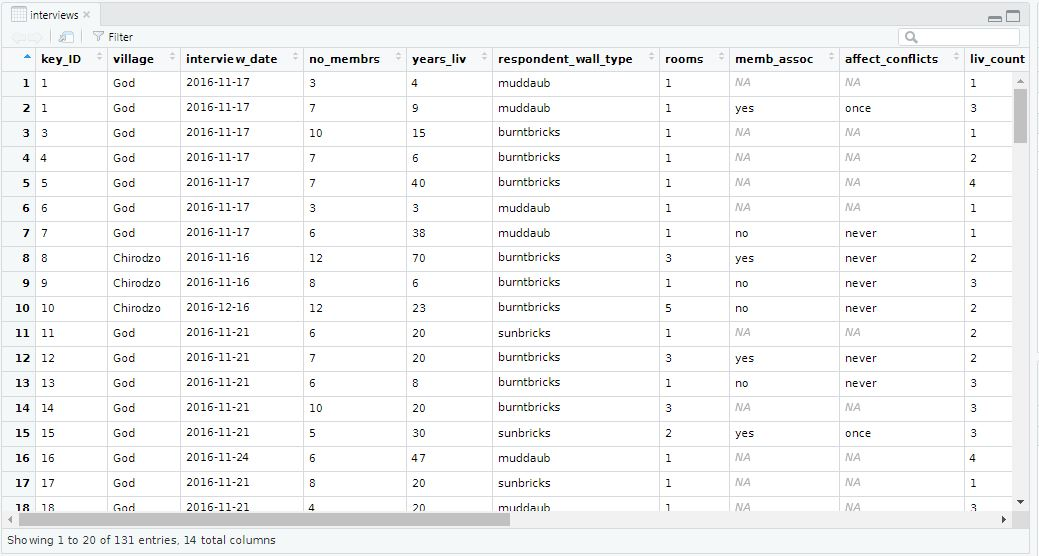
\includegraphics[width=0.8\textwidth]{images/RStudio_01.JPG}
\caption{View(interviews)}
\label{fig:x View(interviews)} 
\end{figure}


Results of the exercise

\begin{figure}[h]
\centering
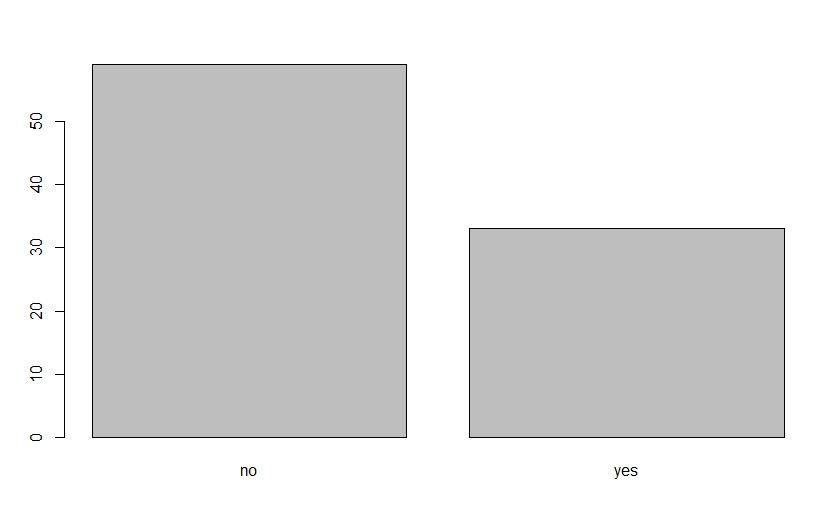
\includegraphics[width=0.8\textwidth]{images/RStudio_02.JPG}
\end{figure}

\newpage
Results
\begin{figure}[h]
\centering
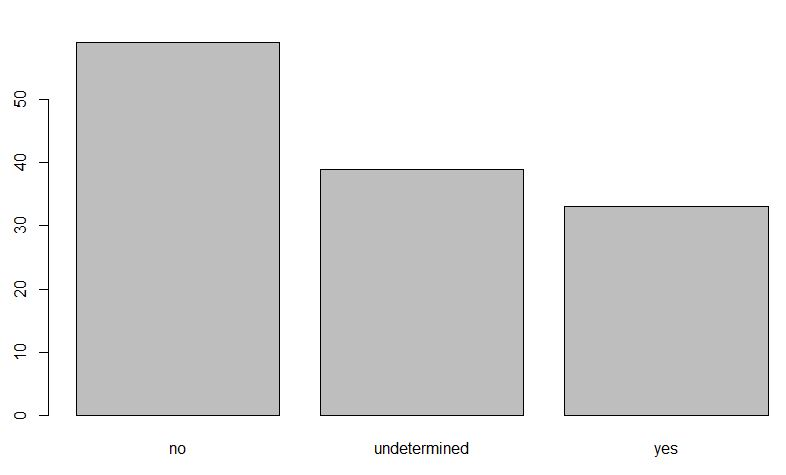
\includegraphics[width=0.8\textwidth]{images/RStudio_03.JPG}
\end{figure}

Results after renaming levels of the factor to have the first letter in uppercase: 
“No”,”Undetermined”, and “Yes” and putting ”Undetermined” last. 

\begin{figure}[h]
\centering
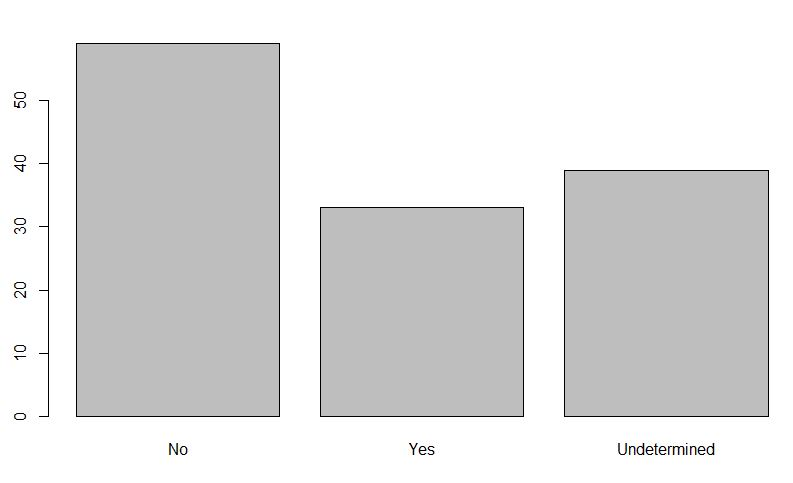
\includegraphics[width=0.8\textwidth]{images/RStudio_04.JPG}
\end{figure}


\subsection{Factors}



\begin{lstlisting}

> respondent_floor_type <- factor(c("earth", "cement", "cement", "earth"))
> levels(respondent_floor_type)
[1] "cement" "earth" 
> nlevels(respondent_floor_type)
[1] 2
> espondent_floor_type # current order
Error: object 'espondent_floor_type' not found
> respondent_floor_type # current order
[1] earth  cement cement earth 
Levels: cement earth
> respondent_floor_type <- factor(respondent_floor_type, levels = c("earth", "cement"))
> 
> respondent_floor_type # after re-ordering
[1] earth  cement cement earth 
Levels: earth cement
> % re-ordered levels, earth first
Error: unexpected input in "% re-ordered levels, earth first"
> # should have been a #
> levels(respondent_floor_type)
[1] "earth"  "cement"
> levels(respondent_floor_type)[2] <- "concrete"
> levels(respondent_floor_type)
[1] "earth"    "concrete"
> # now its says concrete.
> levels(respondent_floor_type)[2] <- "red brick"
> levels(respondent_floor_type)
[1] "earth"     "red brick"
> # testing to see if we can have spaces
> respondent_floor_type
[1] earth     red brick red brick earth    
Levels: earth red brick
> # This is probably not a good practise. Changed to red_brick
> levels(respondent_floor_type)[2] <- "red_brick"
> respondent_floor_type
[1] earth     red_brick red_brick earth    
Levels: earth red_brick

\end{lstlisting}

\subsection{Converting Factors}

\begin{lstlisting}

> as.character(respondent_floor_type)
[1] "earth"     "red_brick" "red_brick" "earth"    
> levels(respondent_floor_type)[2] <- "red brick"
> as.character(respondent_floor_type)
[1] "earth"     "red brick" "red brick" "earth"    
> year_fct <- factor(c(1990, 1983, 1977, 1998, 1990))
> as.numeric(year_fct)  
[1] 3 2 1 4 3
> as.numeric(as.character(year_fct))
[1] 1990 1983 1977 1998 1990
> # exercise says as.numeric(year_fct) is wrong, but what is does is numbered orders.. 1990 is the 3rd in the sequence, 1983 the second etc..
> as.numeric(levels(year_fct))[year_fct]
[1] 1990 1983 1977 1998 1990

\end{lstlisting}

\section{Week 12}

\subsection{Disaster recovery information}

Disaster recovery information is confined to my thesis proper documents and associated files (such as notes, ebooks, papers in pdf format etc.)

\subsubsection{Github}

All of the files for the Proof Of Concept Thesis template are done in Overleaf and are committed to github
\url{https://github.com/a-white42/ProofOfConcept_Thesis_Paper}. This serves the purpose of having tracking in terms of version control and for the purposes of backup in case of an unforeseen disaster in which Overleaf is hacked or stops working. As an addition backup and offline functionality Overleaf is configured to sync with my Dropbox account both as a secondary backup, but also as a means of working offline in a local LaTeX editor in case of internet outage. The Dropbox sync folder is \verb|\Apps\Overleaf\| To work offline, you only need to edit the required document in any LaTeX editor, or any plain text editor (Atom is a good open source text editor, found at \url{https://atom.io/} and when the local Dropbox syncs the Dropbox server the files will automatically sync with Overleaf.   

\subsubsection{Dupliciti}

Secondly, I have Duplicati installed, when I used to backup my other work documents, and this is set to back up all the data located in my Dropbox folder to a an external hard drive and a local hard drive. I backup the Dropbox on a local hard drive just in case the contents of Dropbox is compromised. For example, let as same a hacker deletes files on a local Dropbox and it syncs to all Dropbox drives. All local and online files would have been removed. By having both an external hard drive version and a local version means we can plan for either a hacker or a damaged/lost computer.  

\subsection{In case of disaster: Loss of file, or corruption}
In the worst case of file corruption or a file has gone missing there are several courses of action one could take. 
Both github and Overleaf provides a method of recovering an older files through the version control/history facility.

\subsubsection{Overleaf}

\begin{enumerate}
    \item Select the project in which a file is missing, corrupted, or that you might want to go back to an earlier version.
    \item Select the History tab at the top right of the web interface.
    \item Scroll down until you find the correct file. (you can check by clicking on files to see what the content was on a particular date.)
    \item Select the "download project at this version"
    \item Unzip the file and check the content of the desired file. 
    \item From here we can either copy and paste content into the current online version or upload this file to over-write the current online version.
    
\end{enumerate}


\subsubsection{GitHub}
\begin{enumerate}
    \item go to \url{https://github.com/a-white42/ProofOfConcept_Thesis_Paper}
    \item Select file you want
    \item Select History
    \item You are then presented with a list of every time the file has been committed to github. This emphasises the importance of committing your project regularly.
    \item From here you can search for the older version you might want, or for some text you might want to copy into a newer version. 
    
\end{enumerate}

\subsubsection{Duplicati}
\begin{enumerate}
    \item Open Duplicati
    \item Select restore backup
    \item Select backup to restore or search
    \item Restore files
    
\end{enumerate}

Recovering large quantities of files is beyond the scope of this plan as it involves a lot of time and detail. Duplicati has a disaster recovery page specifically for recovering large numbers of files. 
\url{https://duplicati.readthedocs.io/en/latest/08-disaster-recovery/}

\subsubsection{Overleaf}
Recovering complete project in Overleaf from github. The Thesis Project can be imported into Overleaf, is a worse case scenario where the overleaf project has been deleted or hacked. 
\begin{enumerate}
    \item From the https://www.overleaf.com/project page select 'New Project'
    \item Choose import from github
    \item Select appropriate project (for example, ProofOfConceptThesisPaper)

    
\end{enumerate}

\subsubsection{In case of disaster: New Computer required}
\begin{enumerate}
    \item Install Linux Fedora found at https://getfedora.org/
    
    - boot cd or usb
    
    - partition hard drive or use VLM
    
    - Follow installation prompts
    
    - reboot system after install (10-15 mins)
    
    \item install Dropbox, instructions found at \url{https://www.dropbox.com/install-linux}
    \item Sync Dropbox (this will restore all data from the Dropbox online server)
    \item Update system using \verb|$ sudo dnf update|
    \item Install Firefox (login to enable synchronize bookmarks and history)
    \item Download and install Duplicati for Fedora \url{https://www.duplicati.com/download}
    
    - Install mono for fedora. Mono is an open source implementation of the Microsoft .NET framework. 
    
    - \verb|$ sudo dnf install mono-complete|
    
    - \verb|$ sudo dnf install [name of duplicati file].rpm|
    
    \item install additional software:
    
    - \verb|$ sudo dnf install R|
    
    - \verb|$ sudo dnf install texlive|
    
    - \verb|$ sudo dnf install texlive-biblatex|
    
    - \verb|$ sudo dnf install texmaker|
    
    - \verb|$ sudo dnf install gnome-tweak-tool|
    
    
    \item Login to GitHub and get new computer verification code.
    
\end{enumerate}

\newpage

\section{Week 12}

\subsection{Fancyhdr in Proof Of Concept}

\textbf{Errors:} The Fancyhdr LaTEX package is printing Chapter 0 on the frontmatter pages of my thesis--on the abstract, declaration,  dedication, and acknowledgement pages. The references to chapters should not begin until chapter 1. 

\textbf{Objective:} Find some code to tell LaTeX not to print chapter 0 in the frantmatter.

\textbf{Action:} Searching the internet forums I found a few solutions but the simplest one was to add some code which tells LaTeX only to print the chapter number if it is greater than 0. This code was added to the preample section where I have included the fancyhdr settings. 

\verb|\fancyfoot[LO,CE]{\ifnum \value{chapter}>0 Chapter \thechapter\fi}| 

\textbf{Results:} This was successful and the PDF file complied without chapter 0 printing in the frontmatter. 

\subsection{Annotated Bibliography}

After a lot of revisiting the annotated bibliography and experimenting with some pre-made code, I have returned to a fairly straightforward set up. 

This is the code I am now using in the annotate.tex file in my Proof Of Concept. It reference the same biblatex file as the main thesis document, however, it calls the \verb|annote={}| field and prints this in the \verb|\printbibliography[]|

\begin{verbatim}
\usepackage[notes,backend=biber,isbn=false,annotation]{biblatex-chicago}

\addbibresource{references.bib}

\begin{document}

\maketitle

\nocite{*}

\setlength{\bibitemsep}{1.6\itemsep} 

\nocite{*} 

\printbibliography[title={References}] 

\end{verbatim}


\subsection{Proof Of Concept Testing}

\textbf{Objective:} Test changing document paper sizes. Options, a4paper, executivepaper, legalpaper, a5paper. 

\textbf{Action:} In the preample of the thesis document, change the paper size setting, currently set at a4paper,
\begin{lstlisting}
\usepackage[a4paper, top=25mm, bottom=25mm, bindingoffset=5mm, marginparwidth=2.5cm]{geometry} 
\end{lstlisting}
to a4paper, executivepaper, legalpaper, and a5paper. Generate a pdf file of each options and check results.   

\textbf{Results:}  a4paper, executivepaper and legalpaper paper sizes generated satisfactorily and the results have been uploaded to the Testing folder on Overleaf and GitHub.

\textbf{Errors:} a5 paper created an error due to the paper size width OF a5 paper is 148mm, and the specified width of the text, which is set to 140mm. This only allows 8mm of play, 4mm on each side. I removed the 140mm text width and this fixed the problem. 

%% \subsection{Template Section}
%% \textbf{Objective:}
%% \textbf{Action:}
%% \textbf{Errors:}
%% \textbf{Results:}

\newpage
\nocite{*}
\bibliography{foar705bib.bib}
\bibliographystyle{apalike}

\end{document}